\documentclass{standalone}
\usepackage{tikz}
\usepackage{ctex,siunitx,ninecolors}
\setCJKmainfont{Noto Serif CJK SC}
\usepackage{tkz-euclide}
\usepackage{amsmath}
\usepackage{wasysym}
\usetikzlibrary{patterns, calc}
\usetikzlibrary {decorations.pathmorphing, decorations.pathreplacing, decorations.shapes,}
\begin{document}
\small
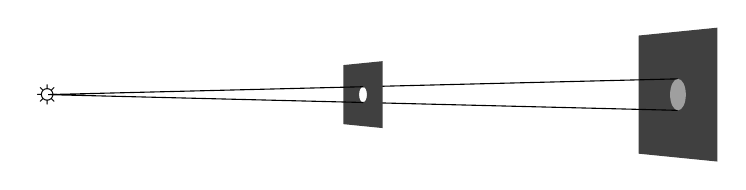
\begin{tikzpicture}[>=latex,scale=1.0]
  \node at (0,0){\sun};
  \fill[darkgray](7.5,0.75)--(7.5,-0.75)--(8.5,-0.85)--(8.5,0.85)--cycle;
  \draw(8,-0.2)--(4,-0.1)(4,0.1)--(8,0.2);
  \fill[darkgray,even odd rule](3.75,0.375)--(3.75,-0.375)--(4.25,-0.425)--(4.25,0.425)--cycle (4,0)ellipse( 0.05 and 0.1);
  \fill[white,opacity=0.5](8,0)ellipse(0.1 and 0.2);
  \draw(4,-0.1)--(0,0)--(4,0.1);
\end{tikzpicture}
\end{document}